\chapter{Discussion}

In this Chapter I will discuss how my results compare to others I have not yet touched upon and discuss their broader implications (Section~\ref{sec:bigpic}). I will then discuss future work with \starpy\ (Section~\ref{sec:future}) and its application to IFU spectral data (Section~\ref{sec:IFU}). I will end with a reflection on the power of Hubble Space Telescope imaging in comparison to SDSS imaging. 

%I will also discuss the implications my results have for the proper use of morphology in galaxy evolution studies (Section~\ref{sec:usemorph}).

\section{The Big Picture}\label{sec:bigpic}

I have investigated quenching as a function of colour, morphology, the presence of an AGN and environmental properties across a large galaxy population. I have found that the green valley is tracing the evolution of the red sequence and that thought here is a morphological dependance on the quenching rate, galaxies of any morphology can quench at any rate (Chapter~\ref{chap:morph}). I have found that those lower mass galaxies hosting an AGN have quenched rapidly and recently, suggesting that AGN may be the direct cause of this quenching (Chapter~\ref{sec:agnfeedback}). However, I have also shown that quenching in AGN host galaxies does not always proceed rapidly, suggesting a slower co-evolution of galaxies with their black holes. I investigated this slower evolutionary path with a sample of bulgeless AGN host galaxies which were found to host black holes which were much more massive than typical black hole scaling relations predict (Chapter~\ref{intbulgeless}). I have also found evidence for mergers, environmentally driven quenching mechanisms, mass quenching and morphology quenching all across the group environment; the derived timescales for which imply that the environmentally driven quenching mechanisms must work in sync to quench a satellite galaxy (Chapter~\ref{chap:env}). I shall now discuss how all of these results fit into the `big picture' of galaxy evolution. 

In Chapter~\ref{chap:morph} I discussed how the results suggested that quenching rates with $\tau < 1.5~\rm{Gyr}$ must be caused by mechanisms which can transform morphology from a disc to an elliptical. However this does not infer an immediate transition from disc dominated to bulge dominated. Work by the \textsc{ATLAS}$^{\rm{3D}}$ team \citep{cappellari11} showed that kinematic discs are found in the majority of the visually elliptical population \citep{emsellem11} with $\sim7$ times the number of \emph{fast rotators} (with kinematic discs) than \emph{slow rotators} \citep[with dispersion dominated kinematics see][]{cappellari07, emsellem07}.  This has led to the proposal of a new morphological classification scheme in the form of a ``comb" \citep{refs}, whereby the evolution of discs from Sd-Sa takes place along the tines of the comb until they become fast rotators, which then evolve off the base of the comb to become slow rotators. Given the nature of the GZ vote fractions, both fast and slow rotators will most likely have been classified as smooth galaxies and so are expected to contribute more to the smooth weighted populations shown in Chapters~\ref{chap:morph} \& \ref{chap:agn}. Below I discuss how this will impact on the conclusions made in Chapter~\ref{chap:morph}. 

Dry major mergers are considered the most likely process to produce fast rotators \citep{duc11, naab14} as they can destroy the disk dominated nature of a galaxy \citep{toomre72} in rapid timescales. I find that across the red sequence population in Figure~\ref{red_s} that $12\%$ of the population density lies below $\tau <0.2 \rm{Gyr}$, in agreement with predictions that between $14-17\pm5\%$ of ellipticals are slow rotators \citep{emsellem11, stott16}, suggesting that these are the quenching rates which might give rise to a slow rotator. This therefore also provides an estimate for the percentage of the galaxy population which have undergone a dry major merger, estimated to be approximately $?\%$ by various observational studies \citep{ref bomb}

Fast rotators are theorised to be formed by the slow build up of a galaxy's bulge over time, until it eventually overwhelms the disc. This growth is thought to occur via gas-rich major and minor mergers \citep{duc11} which can produce a bulge dominated quenched galaxy, which would be visually classified as an elliptical (or a smooth galaxy by GZ users). Until recent times, major mergers were considered the only mechanism which could achieve such a result, however I showed in Chapter~\ref{chap:morph} that in order for the ratio of smooth : disc galaxies in the green valley to match that of the red sequence, all mechanisms with $\tau < 1.5 ~\rm{Gyr}$ must be able to cause a morphological change during quenching. This gradual, relatively slow evolutionary history may help to explain why studies have found that the current major merger rate is much lower than expected given the observed red sequence ($\sim 10\%$, \citealt{Lotz11}). The larger IFU studies of MaNGA, SAMI and CALIFA will allow for larger populations of slow and fast rotators to be identified so that the relative dominance of gas-rich and dry mergers across the elliptical population can be determined more accurately. 

There is also a wealth of literature studying the rare \citep[$<1\%$;][]{Wong12, wild16} `missing link' post-starburst (PSB) galaxy phase. They are thought to have undergone an intense, unsustainable period of star formation in the recent past which has then rapidly quenched \citep{dressler83, abraham96b, poggianti99, goto03, goto05b, goto07}. Such a phase can add a significant fraction \citep[$\sim10\%$;][]{wild10} to the stellar mass of a galaxy and is thought to be linked with merger activity \citep{zabludoff96, blake04, goto05b, yang08, pawlik16}. \citet{Wild09}, who by making assumptions for how long galaxies spend in a PSB phase, estimated that gas rich major merger induced starbursts, which simultaneously cause a morphological change, could account for $38\%$ of the growth of the red sequence at $z\sim0.7$. Figure~\ref{red_s} shows that $\sim40\%$ of the smooth weighted red population undergoes quenching at rates less than $0.7~\rm{Gyr}$, suggesting that these quenching rates could be associated with this post-starburst transition phase. 

However, earlier in this Section, I discussed how these relatively rapid quenching rates were also associated with the production of fast rotators. Work by \citep{pracy13} found that of the 26 `E+A' galaxies with kinematics, 22 ($\sim85\%$) were classed as fast rotators. Although at first this result seems to suggest a connection between the PSB phase and fast rotator production, this fraction is in fact similar to the overall fraction of fast rotators found in the elliptical galaxy population \citep{emsellem11, stott16}. These kinematic studies of galaxies also allow for insights into the locations of recent star formation through spectral indicators of star formation \citep[such as $H\alpha$][]{kennicutt94}. The recent distribution of the first data releases from MaNGA \citep{ref}, SAMI \citep{ref} and CALIFA \citep{ref} will provide a larger sample of PSB galaxies classified as either fast or slow rotators. Using \starpy\ to determine the spatially variant SFHs of these galaxies may help to further disentangle the theorised connection between PSBs and elliptical galaxies and the estimated contribution to the growth to the red sequence by this rare, short-lived, yet perhaps crucial evolutionary phase. 

A galaxy property which I have also overlooked in this work, but which is often investigated in quenching studies, is the stellar mass surface density of a galaxy, which is found to correlate with SFR \citep{barro13b, whitaker16}. As a galaxy's bulge grows it is thought to be able to stabilise a disk against collapse and effectively stop it from forming stars. This is classed as a type of morphological quenching and is effective over a few $\rm{Gyr}$ \citep{Fang13} even if external gas is still fed to a galaxy. This slower quenching track of bulge dominated galaxies may help to explain the slow quenching rates observed across the red and green smooth weighted population densities seen in Figures~\ref{red_s} \& \ref{green_v}. The results in Chapter~\ref{chap:morph} suggest that slower quenching of smooth galaxies is occurring in up to $40\%$ of the smooth weighted red population (see Figure~\ref{red_s}). The processes which both quench and grow the bulge simultaneously (such as a merger or interaction) and those which only grow the bulge and the SFR is consequently lowered slowly by morphological quenching have therefore been separated in the red sequence population densities. However, even in the former case, morphological quenching may help in either speeding up the process or in keeping the galaxy quenched post interaction. This is supported by the finding of \cite{abramson16} who found there is no threshold at which density triggered quenching occurs, but that denser systems typically redden faster than less dense galaxies. This suggests a partnership between minor mergers and morphological quenching is needed to achieve true quiescence, similar to the partnership between starvation and stripping discussed in Chapter~\ref{chap:env}. 

This partnership between two mechanisms is also reminiscent of the idea that without AGN feedback a major merger cannot fully quench a galaxy, as discussed in Chapters~\ref{chap:morph} \& \ref{chap:agn}. Figure~\ref{rate} shows that galaxies in the \textsc{agn-host} population don't always quench at the rapid rates caused by major mergers, suggesting that a slow co-evolution of black hole and host galaxy can occur. Left alone, AGN are only efficient as a quenching mechanism in low mass galaxies where they can have a greater impact. In combination with a major merger however, they can completely quench a massive galaxy and prevent further star formation from occurring \citep{conselice03, springel05b, hopkins08a}. These effects are therefore easily detectable, leading to the initial theories for the links between AGN and mergers \citep{merritt01, hopkins06b, hopkins08a, hopkins08b, peng07, jahnke11}. However, by studying the population as a whole with more robust statistics, the more subtle role of AGN across the population has been revealed. 

Across the galaxy population we now have lots pf examples of two quenching mechanisms working together to either quench a galaxy or ensure a galaxy stays quenched, including starvation and stripping (Section~\ref{sec:roleenv}), mergers \& AGN (Section~\ref{rapid}), disc instabilities \&  environment (Section~\ref{sec:rolemorphenv}) and minor mergers \& morphological quenching (Section~\ref{sec:bigpic}). All of these mechanisms are striving towards the same end goal of galaxy quiescence (with the occasional influx of gas thwarting their progress) but no single mechanism dominates over another, except in the most extreme environments or masses. While mass and morphological quenching will be far more likely to occur in the field, they still impact galaxies in the densest environments. Similarly, mergers will be far more likely to be a part of a galaxy's evolutionary history if it resides in dense environments and will often drown out the more subtle effects of slower quenching mechanisms which occurred before the merger. %The dominance of each mechanism is therefore a matter of circumstance. 

Just as the bulge-to-total ratios of galaxies are continuous in nature, so too are the quenching mechanisms which can cause this change from a disc to a bulge dominated galaxy. The impact of mergers on the morphology and SFR of a galaxy can be measured as a continuum of mass ratios from micro mergers \citep{carlin16} through to major mergers. The strength of morphological quenching mechanisms is a continuum in mass and stellar mass surface density of a galaxy; similarly the impact of environmentally driven quenching mechanisms increases with increasing halo mass. All of these processes, depending on a galaxy's environment, are likely to affect a galaxy at some point in its lifetime, acting in concert to reduce the SFR to produce the wide distribution of quenching timescales seen across the colour-magnitude diagram in Chapter~\ref{chap:morph}. In previous works, efforts have been made to identify the dominant quenching mechanism in a galaxy sample \citep{citebomb}, however it is clear from this work that multiple quenching mechanisms will affect galaxies across their lifetime, working in conjunction to ensure galaxies stay quenched. Future studies should therefore focus on disentangling the effects of these various different quenching mechanisms, rather than focussing on a single process. 

%Rather than focusing on isolating the effects of a single  dominant mechanism, future galaxy evolution studies should attempt to understand this interplay of all possible quenching mechanisms over cosmic time. 

%\section{The use of morphology in large surveys}\label{sec:usemorph}
%
%As discussed in Section~\ref{sec:bigpic}, I consider morphology a continuous spectrum from disc dominated to bulge dominated systems which roughly reflects the continuous nature of galaxy evolution. This continuous nature is reflected by the parameters currently used to characterise the structure of a galaxy, including S\'ersic index \citep{sersic68}, Gini coefficient \citep{abraham03, lotz04}, asymmetry \citep{conselice00} and concentration index \citep{morgan58}. A problem arises however, when studies discretise these values by mapping them to the typical distinct Hubble classifications of morphology; either the data is mapped to T-types \citep{shimasaku01, brinchmann04, barro15} or merely split bimodally into late and early types, e.g. with S\'ersic index, $n \leq 2.5$ to identify discs \citep{ravindranath04, kelvin12, vika15}. Doing so reduces the complex internal structures which encode a galaxy's evolutionary history into two broad bins within which galaxies do not always share common features. This tendency to split populations bimodally is a common trope across the astrophysical community. Although this classification is physically motivated in some cases, such as Cephid variables and planet classification, in other instances this is not the case, e.g. Type 1 and 2 Seyferts, slow and fast rotators, long and short gamma ray bursts, supernova classifications and galaxy morphology, as I argue here. 
%
%It is unsurprising that previous studies of galaxy evolution while split the galaxy population bimodally into early- and late-types galaxies have concluded there are two dominant evolutionary histories \citep[e.g.][]{schawinski14, casado15, belfiore16}. However, I have shown throughout this thesis that this is not the case, finding a continuous distribution of quenching rates across the galaxy population. I believe that this result is possible, in part due to the robust statistical method employed, but also due to the correct use of the full data set which is weighted by the continuous GZ vote fraction estimating the likelihood of either a disc or smooth galaxy. Ideally morphological parameters should be kept in their continuous forms to retain all the information about the galaxy's evolutionary history encoded in its structure \citep[e.g. see work by][]{peth16, savorgnan16, krywult16} For large surveys where a large amount of effort is placed in multi-component fitting \citep{haussler07, haussler11, haussler13, simard11, bruce14, vika15, johnston16} the use of morphology is particularly important as we must understand how to effectively utilise these fits when studying the dependence of morphology on a galaxy's quenching history. I believe that adapting such methods in future studies will allow the `high hanging fruit' science results to be picked out from both archival data and upcoming large surveys, such as LSST \citep{ivezic08}. 
%

\section{Future Work}\label{sec:future}

Due to the flexibility of the \starpy\ package I believe it will have a significant number of future applications. Firstly by investigating quenching using different wavebands as star formation indicators. For example, the $U-V$ and $V-J$ colours are used to separate star forming and quiescent galaxies on the UVJ diagram \citep{labbe05, wuyts07, williams09, brammer11, patel12} at higher redshift (out to $z\sim4$) in the COSMOS/UltraVISTA fields \citep[e.g. see work by][]{muzzin13}. Morphological classifications are also available for the COSMOS field with the recent release of the \textsc{gz:hubble} classifications in \cite{willett16}. With these morphologies, \textsc{popstarpy} can be used to investigate the SFHs inferred by these  UVJ colours for galaxy populations. This will help to further constrain the relative interplay of quenching mechanisms across the galaxy population with cosmic time. 

Secondly, \starpy\ could be adapted to consider many different possible SFHs for a galaxy and examine the Bayesian evidence to chose which is the most appropriate model to characterise the observed photometry of a galaxy. The current exponentially declining SFH (often called the ``$\tau$-model") used in \starpy\ is considered the simplest possible SFH one can assume and so more detail about the effects of different quenching mechanisms may be elucidated by increasing the complexity. For example, possible SFHs include a starburst model \citep{kauffmann03}, an extentded $\tau$-model \citep{simha14}, a Gaussian model \citep{feuillet16} or a log-normal SFR \citep{gladders13, abramson16}. 

Thirdly, improving the\textsc{popstarpy} analysis to use a fully hierarchical Bayesian inference method to determine the parent population parameters. To do this, without inferring a distribution for the unknown shape of the parent distribution, `heat map optimisation' can be used whereby the two dimensional parameter space is split into a grid of pixels (see Section~\ref{althyper}). The values of each pixel then become the hyper Bayesian parameters which describe the population parent posterior distribution and are inferred by randomly sampling from the individual galaxy posterior probability distributions derived by \starpy.  

Along with these expansions of the \starpy\ module itself, several avenues of data exploration are also still available using \starpy\ in it's current form (future work using IFU data are also discussed see Section~\ref{sec:IFU}):
\begin{enumerate}[(i)]

\item A study of barred vs non-barred galaxies using $\{p_{\rm{bar}}, p_{\rm{no bar}}\}$ in place of $\{p_{\rm{disc}}, p_{\rm{smooth}}\}$ to weight the population densities derived with \textsc{popstarpy} may reveal the impact a bar can have on a galaxy's SFR by funnelling gas to central regions.

\item Studying the SFHs of low mass satellite galaxies with $M_* \leq 10^{8-9} ~M_{\odot}$, which are thought to have quenching histories dominated by ram pressure stripping \citep{hester06, fillingham16}, may help to constrain the quenching timescales for this mechanism. However, constructing a large sample of these galaxies may be difficult. Studying such galaxies is difficult as they are only detected in surveys at lower redshifts due to their lower luminosities. 

\item The effect of AGN feedback could be studied further by investigating the SFHs of unobscured Type 1 AGN (however this would require either a more accurate subtraction of the unobscured nuclear emission or a change in the bandpass input to \starpy\ to negate this issue) and those AGN identified by X-ray, radio and IR selection methods.  The results of \citep{ellison16} show that only radio and optically selected AGN have SFRs distributed below the SFS, whereas IR selected AGN have SFRs consistent with the SFS. This suggests that different selection methods may be biased towards either star forming or quenched galaxies. Reproducing the result seen in Chapter~\ref{sec:agnfeedback} with these AGN would corroborate the idea that quenching is actually occurring across the entire AGN population, and provide further support for the theory of AGN unification \citep{antonucci93, urry95}.

\end{enumerate}

\section{The use of \starpy\ with IFU data}\label{sec:IFU}

\begin{figure}
\centering{
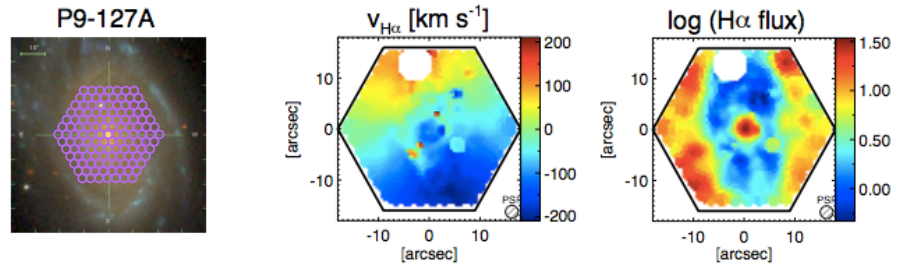
\includegraphics[width=0.95\textwidth]{discussion/manga_data.png}}
\caption[Example MaNGA fibre bundle on a target galaxy with example emission data]{Example fibre bundle placed over a MaNGA target galaxy (left) and corresponding preliminary survey data showing the mapped velocity (middle) and flux (right) of $H\alpha$ gas emission as measured across the galaxy in each fibre. Such measurements can be utilised to calculate the star formation rate across the structure of a galaxy. Adapted from \cite{bundy15} Figure 14.}
\label{fig:manga}
\end{figure}

In Chapter \ref{chap:agn} I discussed how the current SDSS data (both photometric and spectroscopic) cannot determine whether the AGN is the cause or the consequence of the quenching seen across the AGN host population in Figures \ref{time} \& \ref{rate}. Using data from the MaNGA IFU survey \citep{bundy15} I hope to determine whether feedback from the AGN is truly the cause of this quenching. The MaNGA survey will provide 127 spectra across a single galaxy (see Figure~\ref{fig:manga}), allowing the SFH to be mapped as a function of radius. The acquisition of a spectrum in each of these apertures allows for the modification of \starpy\ to take spectral star formation indicators \citep[such as $H\alpha$][]{kennicutt94} to break the degeneracy provided by the photometric colours (see Figure~\ref{pred}), and also the easy removal of any unobscured AGN in the central regions. 

Any correlation of the inferred quenching parameters with radius of the galaxy will allow the determination of whether quenching is happening from the outside-in \citep[i.e. due to the environment, as in][]{pan15, clarke16, schaefer17} or inside-out, as in work with preliminary MaNGA survey data by \citet{belfiore16} and with CALIFA data by \citet{gonzalez16}. I will investigate how this preference for outside-in or inside-out quenching is correlated with the presence of an AGN and a galaxy's environment. This will no only help to answer the question of \emph{cause} vs. \emph{consequence} but also further constrain the timescales of quenching mechanisms possibly caused by AGN or environment. 

A comparison of a large population of fast and slow rotators would aid in the understanding of the different quenching timescales of and interplay between gas-rich and dry major mergers. Although current samples are small, with the first data releases of MaNGA, SAMI and CALIFA a larger sample becomes a possibility. 

There is therefore a lot of work to be done. Investigating all of the proposed ideas in this and the previous Section will take years. However, what I have established in this thesis is a good base on which to build upon with this new influx of IFU data. I have found that

\section{Just one more thing...}\label{sec:hst}

In Chapter~\ref{chap:agn}, I discussed how accurate fits to the bulge-to-total ratio could not be made for galaxies of the \textsc{bulgeless} sample hosting AGN due to the resolution of ground based SDSS imaging. This led to the derivation of upper limits on the bulge masses of this sample. The Hubble Space Telescope (HST) however, provides (i) an extremely stable and well understood point spread function, enabling reliable separation of the AGN from the host galaxy, and (ii) high spatial resolution which is needed to distinguish between classical, merger driven bulges and pseudo bulges grown by secular processes. Observations with the HST of the galaxies in the \textsc{bulgeless} sample will enable extremely robust measures of bulge-to-total ratios for each host galaxy and allow the identification of truly secular systems with growing black holes. Such measurements will also allow the interplay between merger driven (building classical bulges) and merger free (growing pseudo-bulges or retaining a pure disc) co-evolutionary histories to be disentangled. 

\begin{figure*}
\centering{
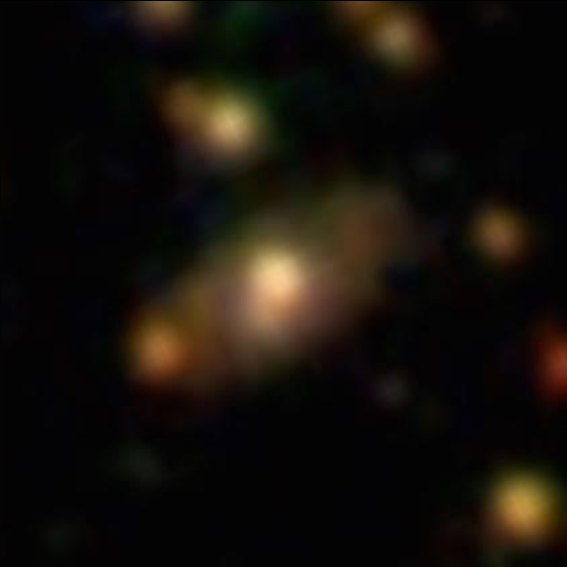
\includegraphics[width=0.49\textwidth]{discussion/sdss_data.png}
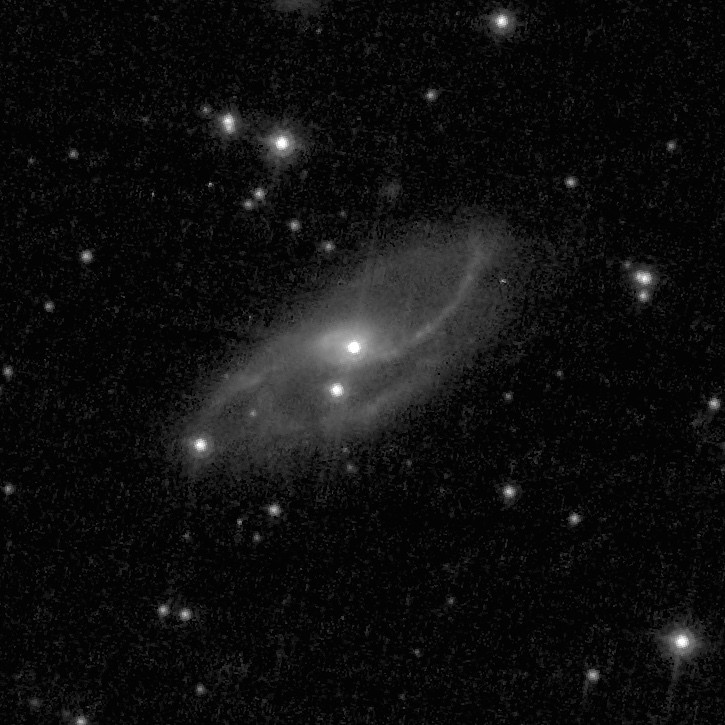
\includegraphics[width=0.49\textwidth]{discussion/hst_data.jpg}}
\caption[Example HST image data in comparison to SDSS]{Example SDSS urgiz image (left) for J$192250.74$-$055259.15$, part of the \textsc{bulgeless} sample, described in Section~\ref{sec:selectAGN}, in comparison to space based imaging from the HST (right). The higher resolution HST image reveals finer structure than the SDSS image, including spiral arms, a ring and a possible bar along with the true disc dominated nature of the galaxy.}
\label{fig:hstdata}
\end{figure*}

We received image data from the HST (Proposal ID: 14606, Cycle 24) of the galaxy J$192250.74$-$055259.15$ from the \textsc{bulgeless} sample on October 26th 2016, on which date I was writing Section~\ref{sec:bulgeless} of this thesis. Figure~\ref{fig:hstdata} demonstrates the difference in resolution provided by the HST with this first image received (right), in comparison with the ground based SDSS ugriz image (left; also shown in Figure~\ref{fig:INTimages}). This galaxy has an estimated black hole mass of $M_{\rm{BH}} = 10^{7.4\pm0.1}~M_{\odot}$ but a bulge-to-total ratio could not be derived from the SDSS image. The HST image will allow for an accurate derivation of the bulge mass of this galaxy, allowing for a more concrete conclusion to be drawn on the controversial issue of secularly driven galaxy-black hole co-evolution. 

